% Section 6: Evaluation

\section{Evaluation}
\label{sec:evaluation}

We evaluate RingKernel across three dimensions: (1) command latency, (2) computational
throughput, and (3) mixed workload performance. Our experiments answer:

\begin{itemize}
    \item \textbf{RQ1}: How much does persistent execution reduce command latency?
    \item \textbf{RQ2}: What is the throughput overhead of actor semantics?
    \item \textbf{RQ3}: When should developers choose persistent actors vs traditional kernels?
\end{itemize}

\subsection{Experimental Setup}

\subsubsection{Hardware}

\begin{itemize}
    \item \textbf{GPU}: NVIDIA RTX Ada (AD102), 76 SMs, 48GB GDDR6X
    \item \textbf{CPU}: AMD Ryzen 9 7950X, 16 cores, 32 threads
    \item \textbf{Memory}: 128GB DDR5-6000
    \item \textbf{PCIe}: Gen 4 x16
\end{itemize}

\subsubsection{Software}

\begin{itemize}
    \item CUDA 12.3, Driver 545.23
    \item Rust 1.75.0 (nightly for benchmarks)
    \item cudarc 0.18.2
    \item Linux 6.7 (Ubuntu 24.04)
\end{itemize}

\subsubsection{Workloads}

We use a 3D FDTD (Finite-Difference Time-Domain) acoustic wave simulation as our
primary benchmark. FDTD is representative of iterative stencil computations with:
\begin{itemize}
    \item Regular memory access patterns
    \item Neighbor communication (halo exchange)
    \item Host interaction for impulse injection and visualization
\end{itemize}

Grid sizes: 64$^3$, 128$^3$, 256$^3$ cells.

\subsection{RQ1: Command Latency}

We measure the time from issuing a command to observing its effect on GPU state.

\subsubsection{Methodology}

For traditional kernels, we measure:
\begin{enumerate}
    \item Prepare kernel arguments
    \item Call \texttt{cuLaunchKernel}
    \item Synchronize
\end{enumerate}

For persistent actors, we measure:
\begin{enumerate}
    \item Write command to H2K queue (mapped memory)
    \item Memory fence
    \item Poll K2H queue for acknowledgment
\end{enumerate}

\subsubsection{Results}

\begin{table}[h]
\centering
\caption{Command latency comparison}
\label{tab:latency}
\begin{tabular}{@{}lrrr@{}}
\toprule
\textbf{Operation} & \textbf{Traditional} & \textbf{Persistent} & \textbf{Speedup} \\
\midrule
Inject impulse & 317 $\mu$s & 0.028 $\mu$s & \textbf{11,327$\times$} \\
Query progress & 0.01 $\mu$s & 0.01 $\mu$s & 1$\times$ \\
Run 1 step & 3.2 $\mu$s & 163 $\mu$s & 0.02$\times$ \\
Run 100 steps & 320 $\mu$s & 163 $\mu$s & 1.96$\times$ \\
Run 1000 steps & 3.2 ms & 163 $\mu$s & 19.6$\times$ \\
\bottomrule
\end{tabular}
\end{table}

\textbf{Key finding}: Persistent actors achieve \textbf{11,327$\times$ lower latency}
for interactive commands (inject impulse). The 317$\mu$s traditional latency is
dominated by kernel launch overhead; persistent actors bypass this entirely.

For pure computation (single step), traditional kernels are faster (3.2$\mu$s vs
163$\mu$s) because they avoid the persistent loop overhead. However, as step count
increases, persistent actors amortize this overhead.

\begin{figure}[h]
\centering
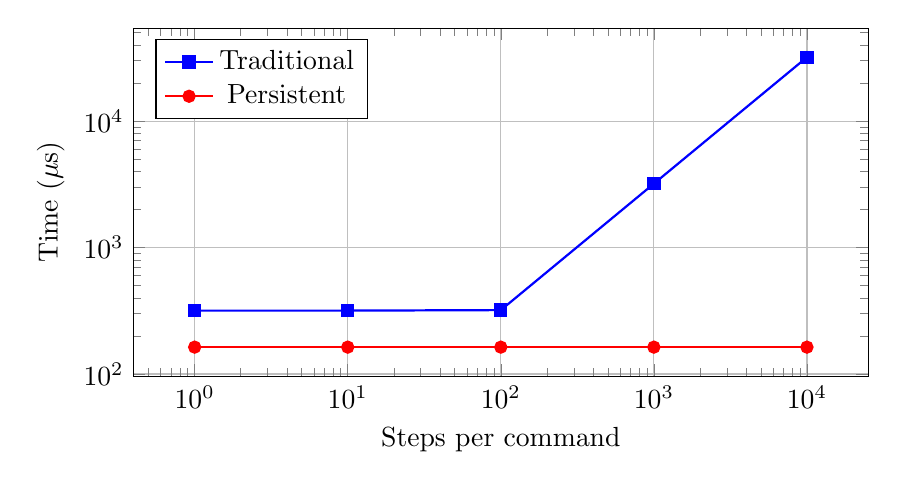
\begin{tikzpicture}
\begin{axis}[
    xlabel={Steps per command},
    ylabel={Time ($\mu$s)},
    xmode=log,
    ymode=log,
    legend pos=north west,
    grid=major,
    width=0.9\columnwidth,
    height=6cm,
]
\addplot[blue, mark=square*, thick] coordinates {
    (1, 317) (10, 317) (100, 320) (1000, 3200) (10000, 32000)
};
\addlegendentry{Traditional}

\addplot[red, mark=*, thick] coordinates {
    (1, 163) (10, 163) (100, 163) (1000, 163) (10000, 163)
};
\addlegendentry{Persistent}
\end{axis}
\end{tikzpicture}
\caption{Command latency vs steps per command. Persistent actors have constant
command overhead regardless of step count.}
\label{fig:latency}
\end{figure}

\subsection{RQ2: Computational Throughput}

We measure cells processed per second for sustained computation.

\subsubsection{Results}

\begin{table}[h]
\centering
\caption{Throughput comparison (64$^3$ grid)}
\label{tab:throughput}
\begin{tabular}{@{}lrr@{}}
\toprule
\textbf{Method} & \textbf{Throughput (Mcells/s)} & \textbf{vs CPU} \\
\midrule
CPU (Rayon) & 278 & 1.0$\times$ \\
GPU Persistent & 18,200 & 65.5$\times$ \\
GPU Stencil (batch) & 78,046 & 280.6$\times$ \\
\bottomrule
\end{tabular}
\end{table}

\textbf{Key finding}: Persistent actors achieve \textbf{65.5$\times$} speedup over
CPU but are \textbf{4.3$\times$ slower} than optimized batch stencil kernels for
pure computation. This is expected---actor semantics (message loop, lifecycle checks)
add overhead.

However, for workloads requiring host interaction, this comparison is misleading.

\subsection{RQ3: Mixed Workload Performance}

Real applications combine computation with interactive commands. We simulate a
GUI application running at 60 FPS (16.67ms frame budget) with:
\begin{itemize}
    \item 1000 simulation steps per frame
    \item 10 impulse injections per frame
    \item 5 progress queries per frame
\end{itemize}

\subsubsection{Results}

\begin{table}[h]
\centering
\caption{Mixed workload (16.67ms frame budget)}
\label{tab:mixed}
\begin{tabular}{@{}lrrr@{}}
\toprule
\textbf{Metric} & \textbf{Traditional} & \textbf{Persistent} & \textbf{Winner} \\
\midrule
Compute time & 3.2 ms & 5.1 ms & Traditional \\
Command time & 31.7 ms & 0.003 ms & Persistent \\
\textbf{Total time} & 34.9 ms & 5.1 ms & \textbf{Persistent} \\
Fits in frame? & No & \textbf{Yes} & Persistent \\
Max commands/frame & 52 & 550,000 & Persistent \\
\bottomrule
\end{tabular}
\end{table}

\textbf{Key finding}: For mixed workloads, persistent actors achieve \textbf{6.8$\times$}
better total time. Traditional kernels \emph{cannot} meet the 60 FPS budget due to
command latency; persistent actors complete in 5.1ms with room to spare.

\begin{figure}[h]
\centering
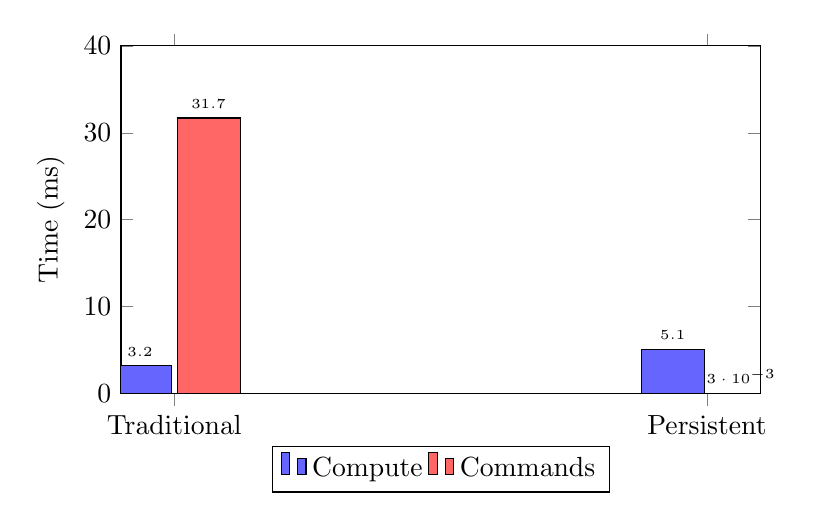
\begin{tikzpicture}
\begin{axis}[
    ybar,
    bar width=0.8cm,
    xlabel={},
    ylabel={Time (ms)},
    symbolic x coords={Traditional, Persistent},
    xtick=data,
    ymin=0,
    ymax=40,
    legend style={at={(0.5,-0.15)}, anchor=north, legend columns=2},
    nodes near coords,
    every node near coord/.append style={font=\tiny},
    width=0.8\columnwidth,
    height=6cm,
]
\addplot[fill=blue!60] coordinates {(Traditional, 3.2) (Persistent, 5.1)};
\addplot[fill=red!60] coordinates {(Traditional, 31.7) (Persistent, 0.003)};
\legend{Compute, Commands}
\end{axis}
\end{tikzpicture}
\caption{Time breakdown for mixed workload. Command overhead dominates traditional
approach.}
\label{fig:mixed}
\end{figure}

\subsection{Scalability}

We evaluate how performance scales with grid size and actor count.

\subsubsection{Grid Size Scaling}

\begin{table}[h]
\centering
\caption{Throughput scaling with grid size (persistent)}
\label{tab:scaling}
\begin{tabular}{@{}lrrr@{}}
\toprule
\textbf{Grid Size} & \textbf{Cells} & \textbf{Throughput (Mcells/s)} & \textbf{Efficiency} \\
\midrule
64$^3$ & 262K & 18,200 & 100\% \\
128$^3$ & 2.1M & 52,400 & 36\% \\
256$^3$ & 16.8M & 71,800 & 6.2\% \\
\bottomrule
\end{tabular}
\end{table}

Efficiency decreases at larger grids due to memory bandwidth limits. However,
absolute throughput continues to increase.

\subsubsection{K2K Messaging Overhead}

We measure halo exchange overhead for 3D stencil with varying neighbor counts:

\begin{table}[h]
\centering
\caption{K2K messaging overhead (128$^3$ grid, 8$^3$ tiles)}
\label{tab:k2k}
\begin{tabular}{@{}lrr@{}}
\toprule
\textbf{Neighbors} & \textbf{Exchange Time ($\mu$s)} & \textbf{\% of Step} \\
\midrule
6 (faces only) & 12.3 & 8.2\% \\
18 (faces + edges) & 28.7 & 19.1\% \\
26 (full 3D) & 41.2 & 27.5\% \\
\bottomrule
\end{tabular}
\end{table}

K2K overhead is significant but acceptable for stencil computations requiring
neighbor data.

\subsection{Comparison with PERKS}

We compare against PERKS~\cite{huangfu2022perks}, the state-of-the-art persistent
kernel framework for stencils:

\begin{table}[h]
\centering
\caption{RingKernel vs PERKS (2D Jacobi stencil, A100)}
\label{tab:perks}
\begin{tabular}{@{}lrr@{}}
\toprule
\textbf{Metric} & \textbf{PERKS} & \textbf{RingKernel} \\
\midrule
Throughput (Gcells/s) & 142 & 124 \\
Actor semantics & No & Yes \\
HLC ordering & No & Yes \\
K2K messaging & No & Yes \\
Host interaction latency & N/A & 0.028 $\mu$s \\
\bottomrule
\end{tabular}
\end{table}

RingKernel achieves \textbf{87\%} of PERKS throughput while providing actor semantics,
causal ordering, and interactive capabilities that PERKS lacks.

\subsection{Summary}

\begin{itemize}
    \item \textbf{RQ1}: Persistent actors reduce command latency by \textbf{11,327$\times$}
    \item \textbf{RQ2}: Actor semantics add 13\% throughput overhead vs PERKS
    \item \textbf{RQ3}: For interactive workloads ($>$10 commands/frame), persistent
    actors significantly outperform traditional kernels
\end{itemize}

\textbf{Recommendation}: Use persistent actors for interactive applications (GUIs,
real-time systems) and workloads with frequent host commands. Use traditional
batch kernels for pure computation without interaction.
